\chapter{The inverse problem of electrocardiography}
%In this chapter I will firstly give a short introduction of the biological background, which makes it possible to measure a potential difference between two electrodes on the torso surface. As the heart with its electro-chemical activity dominates these measurements, I will give a short overview over the anatomy and give an insight into the hearts smallest functional unit, the heart muscle cells. Furthermore a short introduction into the electrocardiography is given, TODO

% Shortly what is inverse problem, and explanation of terminology.
In broad terms, the inverse problem of electrocardiography (iECG) is about gaining knowledge about the activity of the heart, based on measurements from electrodes on the torso surface \cite[p.300]{iECG} Based on this definition, the experiment described below can also be understood as the processing of the inverse problem of ECG. The aim of this study is to find out to what extent it is possible to differ between several pattern in the heart's activity through ECG measurements. 

One of the most important use case of ECG measurements is the classification of the corresponding activity of the heart. [...]
A much more difficult task is the complete reconstruction of the cardiac activity or the surface activity using the ECG signals. Mathematically, this can be described as ill-posed, which in our case means that a possible solution is not unique\footnote{According to the definition of Jacques Hadamard [CITE] a problem is well-posed if (1.) a solution exist, (2.) the solution is unique, and (3.) the solution depends continuously on the data. A problem is ill-posed if it fails to satisfy one or more of these conditions}.
[...]
Therefore, it can be said that the inverse problem of electrocardiography is an important topic in medicine which potential is not yet exhausted.
%In this experiment 
%The aim of this study is to find out to what extent it is possible to quantitatively characterize a structure, by locating the source of concentric waves originating on the heart surface, based on ECG measurements. The data are based on the simulation of the electrical activity of a porcine heart and corresponding ecg signals.

%The terminology inverse indicates that there is a 'forward' problem of ECG. 

%While within the inverse problem, the potential differences at the torso are tried to trace back (inverse) to its source, the forward direction is regarded as the computation of the electric potential 

%as the tracing back of the activity to gain information of the heart's behavior, without directly measuring on its surface.

%The term “forward problem of electrocardiography” is used to denote the computation of the electric potential field generated by cardiac excitation within and on the torso surface.

%The terminology inverse indicates that there is a 'forward' problem of ECG.

%The mathematical description of the propagation of the electrical signals which are coming from the heart and are propagating through the body onto the body surface, is described as 'forward'. The forward propagation is measurable through potential differences between two electrodes on the torso.

%The terminology inverse indicates that there is a 'forward' problem of ECG. The formulation is based on the fact that the electro-chemical activity of the heart is measurably 

%Since the electro-chemical activity of the heart is measurable 

%The terminology inverse indicates that the measurements have 
%The terminology inverse indicates that there is a forward direction. 
\section{Problem formulation}
% Was in etwa
As already briefly explained, this experiment is about the differentiation of activities of the heart, which are characterized by different spatio-temporal excitation patterns. A representation of this activity is provided by the measurements of electrodes at a certain distance from the heart.

% Wie wird es verwirklicht
In this experiment, the data of the electrical activity of the heart as well as the corresponding ECG signals through the electrodes are simulated (see section \ref{cap:simulation} for more details about the simulation). It is a simulation of a pig's heart whose geometric shape comes from a CT-scan. The electrodes are set up at a certain distance within two grids as visualized in figure (\ref{fig:heart_overview}). Four electrodes are marked in the graphic from which a virtual reference electrode is calculated whose geometric center lies approximately in the middle of the heart. All electrodes of the two grids have the same reference electrode.

% Wie wird das Problem verwirklicht
Different excitation patterns are generated by stimulating a previously defined point on the heart surface at a constant frequency, where the position varies in every simulation. This pacing induces a concentric waves which spreads over the entire heart. The aim of this experiment is to predict the position where the pacing events are happening, based on the ECG-signals.

% Daten und was damit angestellt wird.
A simulation generates ECG data in the form $X_{\text{ECG}}\in\mathrm{R}^{T\times N}$ where $T$ is the number of discrete time steps and $N=70$ the number of leads (respectively electrodes, each lead is built with the same virtual electrode). The exact spatio-temporal activity of the heart is not recorded as it is not relevant for the prediction. Only the position of the pacing is stored as a 3-dimensional vector. The selection of the relevant parameters $T$, $N$ and the conversion of the discrete quantities (time and space) into characteristic quantities are described in chapter \ref{cap:simulation} (simulation) respectively \ref{cap:processing} (data processing). 

% Was macht man mit den Daten
%To pose the problem to an algorithm, the 


\begin{figure}[ht]
    \center
    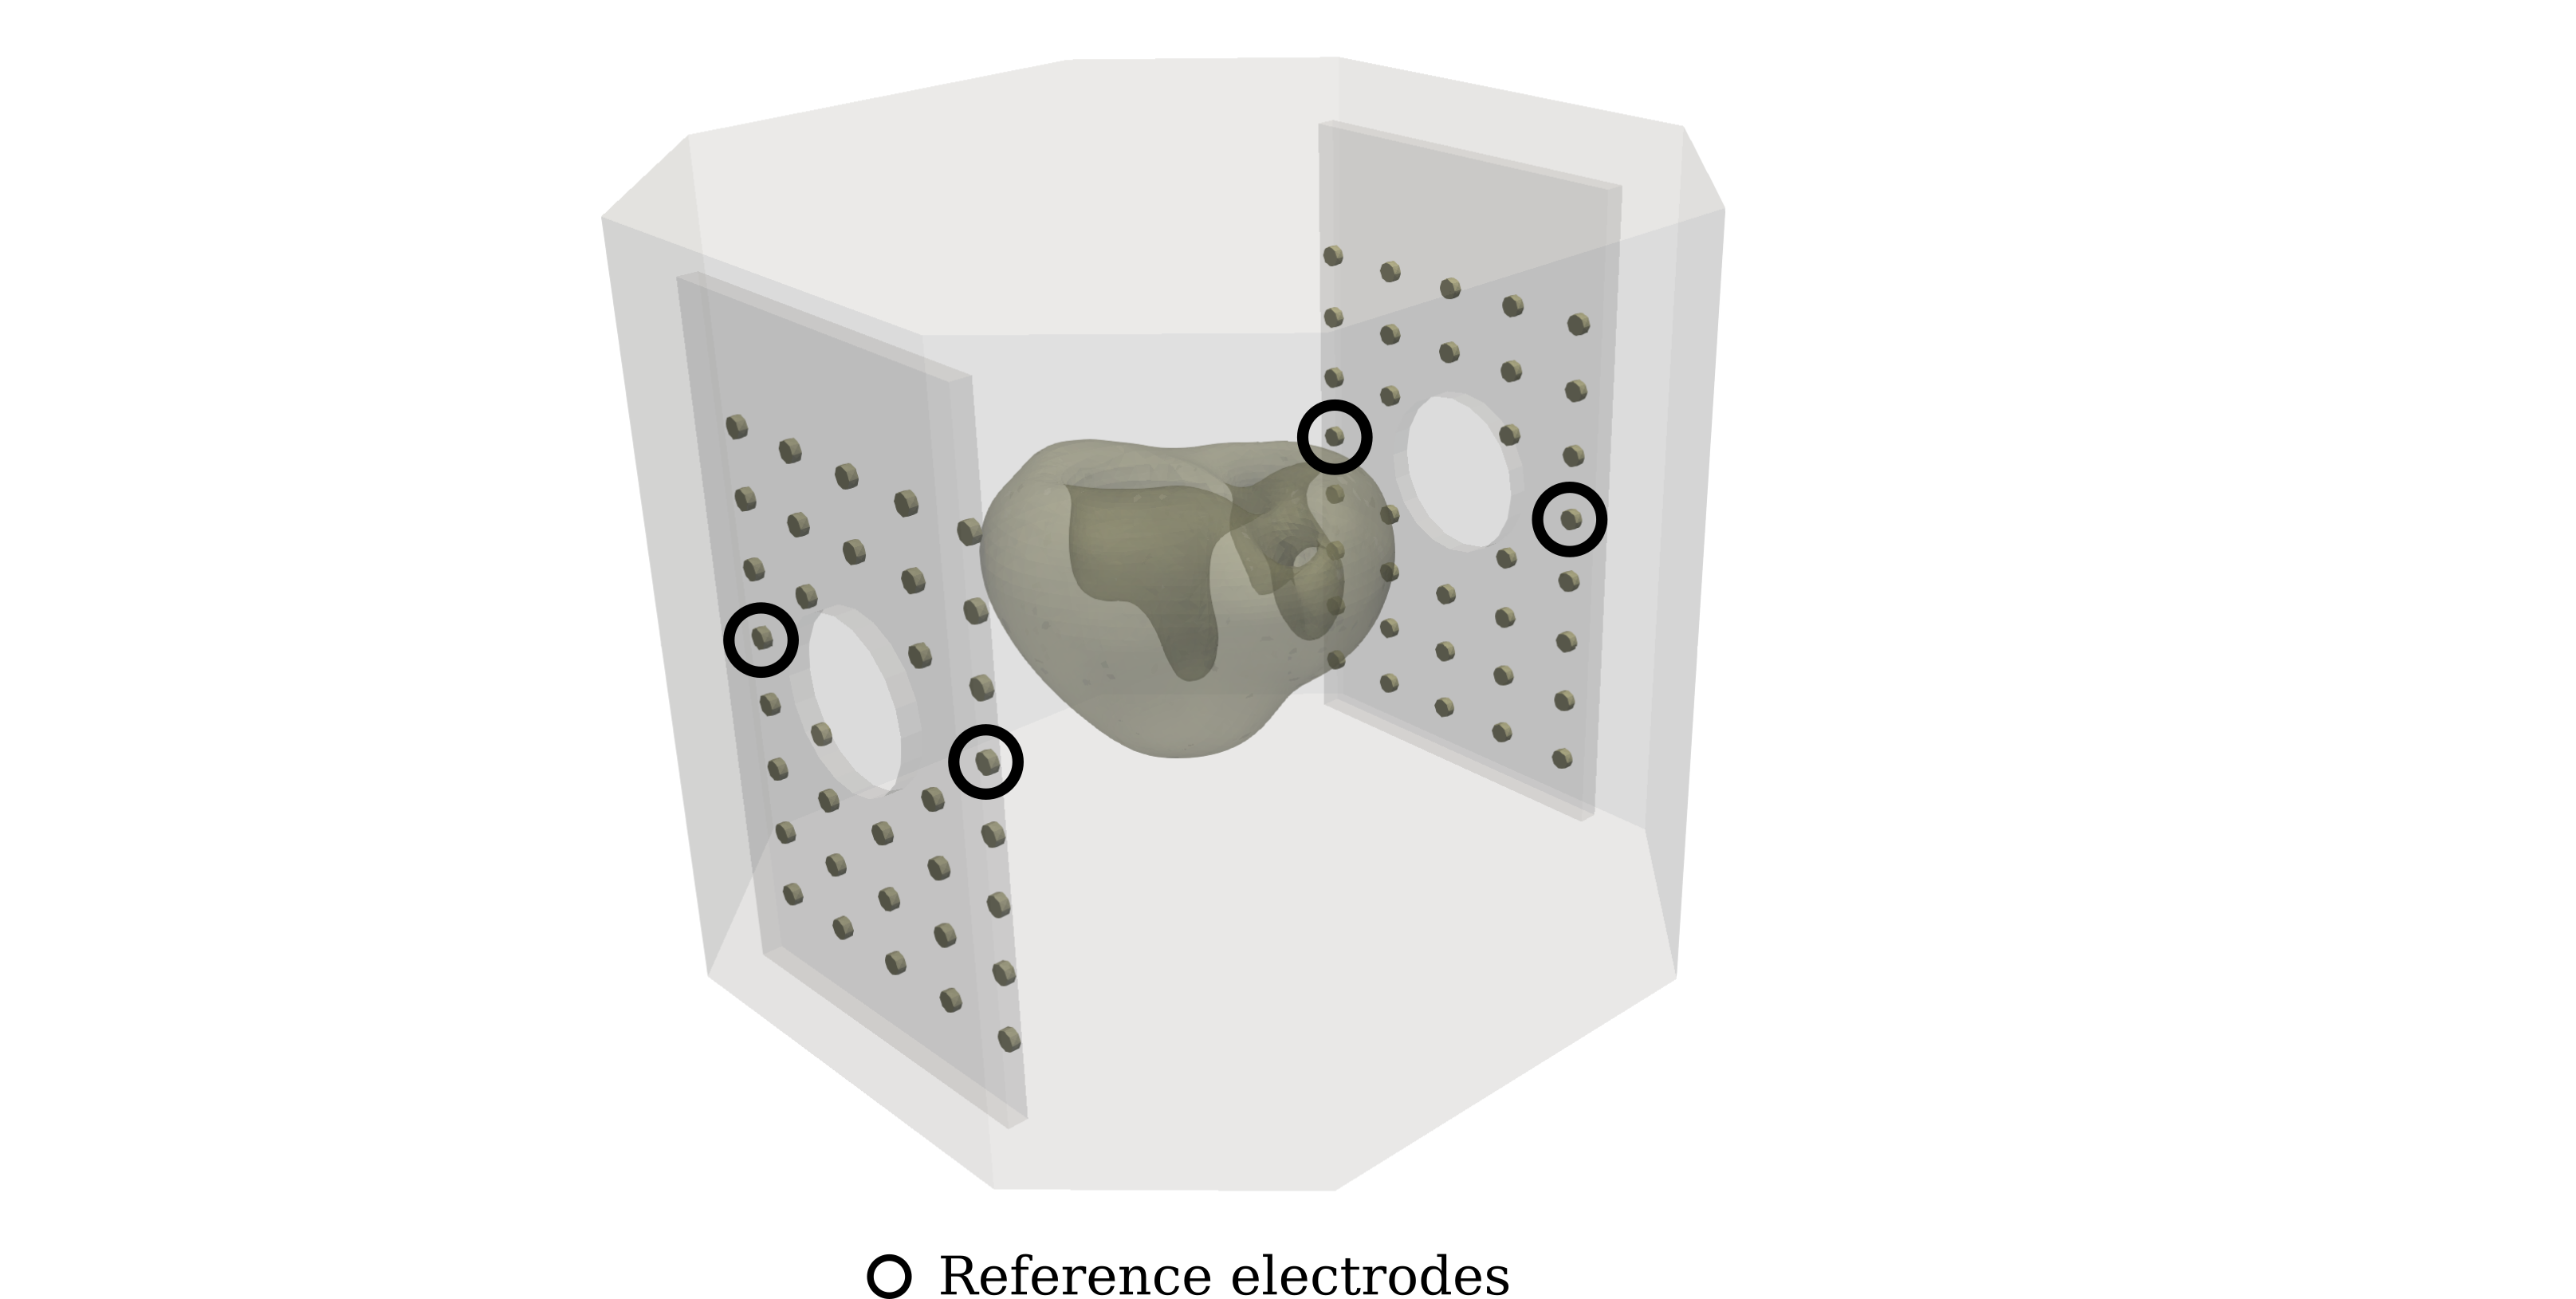
\includegraphics[width=1.3\textwidth]{figures/heart_overview_inkscape.png}
	\caption{Easy}
	\label{fig:heart_overview}
\end{figure}


%As already briefly explained, this experiment is about the differentiation of dynamics in the form of the electrical activity of the heart. The starting point for generating different types of dynamics is an unexcited heart. During the simulation, a point on the heart surface is stimulated with a constant frequency, from which a concentric wave spreads over the entire heart. What an excitation means in this context is described in chapter xx, as well as the biological mechanisms of electrical stimuli transmission so that a concentric wave can arise is described in chapter yy. 
%The location of the stimulation is varied in a number of simulations. the corresponding ECG signals are the input of a neural network, which is supposed to predict the exact location of the stimulation.


%It provides a multi channel-ECG 
%The problem 
%he aim of this study is to find out to what extent it is possible locating the source of concentric waves originating on the heart surface. 
%The data are based on the simulation of the electrical activity of a porcine heart and corresponding ecg signals.
% What is the problem in this work

% why is it important?

\subsection{Related work}
% A few paper
% Problems
\textcolor{red}{A few paper, problems}

% Leserorientierung 
Since the experiment involves the simulation of electrical propagation in cardial tissue, the biological background is first explained in the following chapter. 
%In the following chapter I will give a brief overview of the biological background behind the simulations. This includes the functionality of the heart and the technique of measuring its activity indirectly, the electrocardiography (ECG).


%\textcolor{red}{This numerical experiment tries to find the source of a induced concentric wave, based on multiple ECG signals. The input is multi-channel time-series with dimension $R^{N\times T}$ The output is a 3d-coordinate $\in R^{3}$, therefore the problem is a regression.}

\section{Biological background}
This chapter gives an overview of the anatomy of the heart and its smallest functional units, the cardiac muscle cells. The coordinated contraction of these cells leads to a pumping action of the heart. Within a repetitive pumping process, blood is enriched with oxygen within a heart chamber and passed on to the body. In the following I briefly explain how the anatomy of the heart makes this process possible, as well as discuss the electro-chemical properties of cardiac muscle cells, to understand its coordinated contraction through signal propagation which lead to the pumping effect.

%The mathematical description of the propagation of the electrical signals which are coming from the heart and are propagating through the body onto the body surface, is described as 'forward'. The forward propagation is measurable through potential differences between two electrodes on the torso. In following, I will explain the electro-chemical characteristics of the heart and its spatio-temporal behavior. In the terminology in which the mapping from the activity of the heart to a distant medium (like the torso) is described as forward problem, the inverse problem is defined as the tracing back of the activity to gain information of the heart's behavior, without directly measuring on its surface.

%What is the basis of the heart
% (Leserorientierung: Physiology, heart muscle cells)
\subsubsection{Anatomy of the heart}
This section is based on chapter 1 of the book \textit{Herz-Kreislauf} by J. Steffel and  T. Lüscher \cite{kreislauf}.
The heart consists of four chambers, the left and the right atrium and the left and the right ventricle, as visualized in figure (\ref{fig:heart_anatomy}). The right atrium with the right ventricle builds the right half of the heart, which pumps the blood to the lungs for a gas exchange. From there the blood flows towards the left half of the heart (which consists of the left atrium and the left ventricle). The left half of the heart pumps the oxygen-rich blood towards the individual organs. The heart beats between 50 and 80 times a minute in normal condition. The pumping is caused by an electrical impulse, initiated by the sinus node. The pulse (action potential) is a rapid potential change of the membrane potential induced by moving ions through the cell membrane. The pulse propagates from the atria to the ventricles via the atrioventricular node. The electrical signal causes the cells to contract. In addition, these cells are able to transmit the signal to neighboring cells. In the following I explain the details about the signal transmission.
%Each ventricle represents a separate pump system, nevertheless it forms a unit whose pumping action is based on coordinated muscle contraction initiated by the sinus node. The sinus node in the right atrium initiates pacing signals with action potential. It does not only initiate the contraction, it also sets the pulse speed. The atrioventricular node (AV node) acts as an electrical gateway to the ventricles with controlling the signal propagation of electrical impulses. It ensures that the ventricles are completely filled before the signal from the sinus node initiates a contraction. An effective pumping action comes from the coordinated contraction of single cardiomyocytes. Their electro-chemical neighbor-wise communication leads to a signal which propagates through the heart muscle.

\begin{figure}[ht]
    \center
    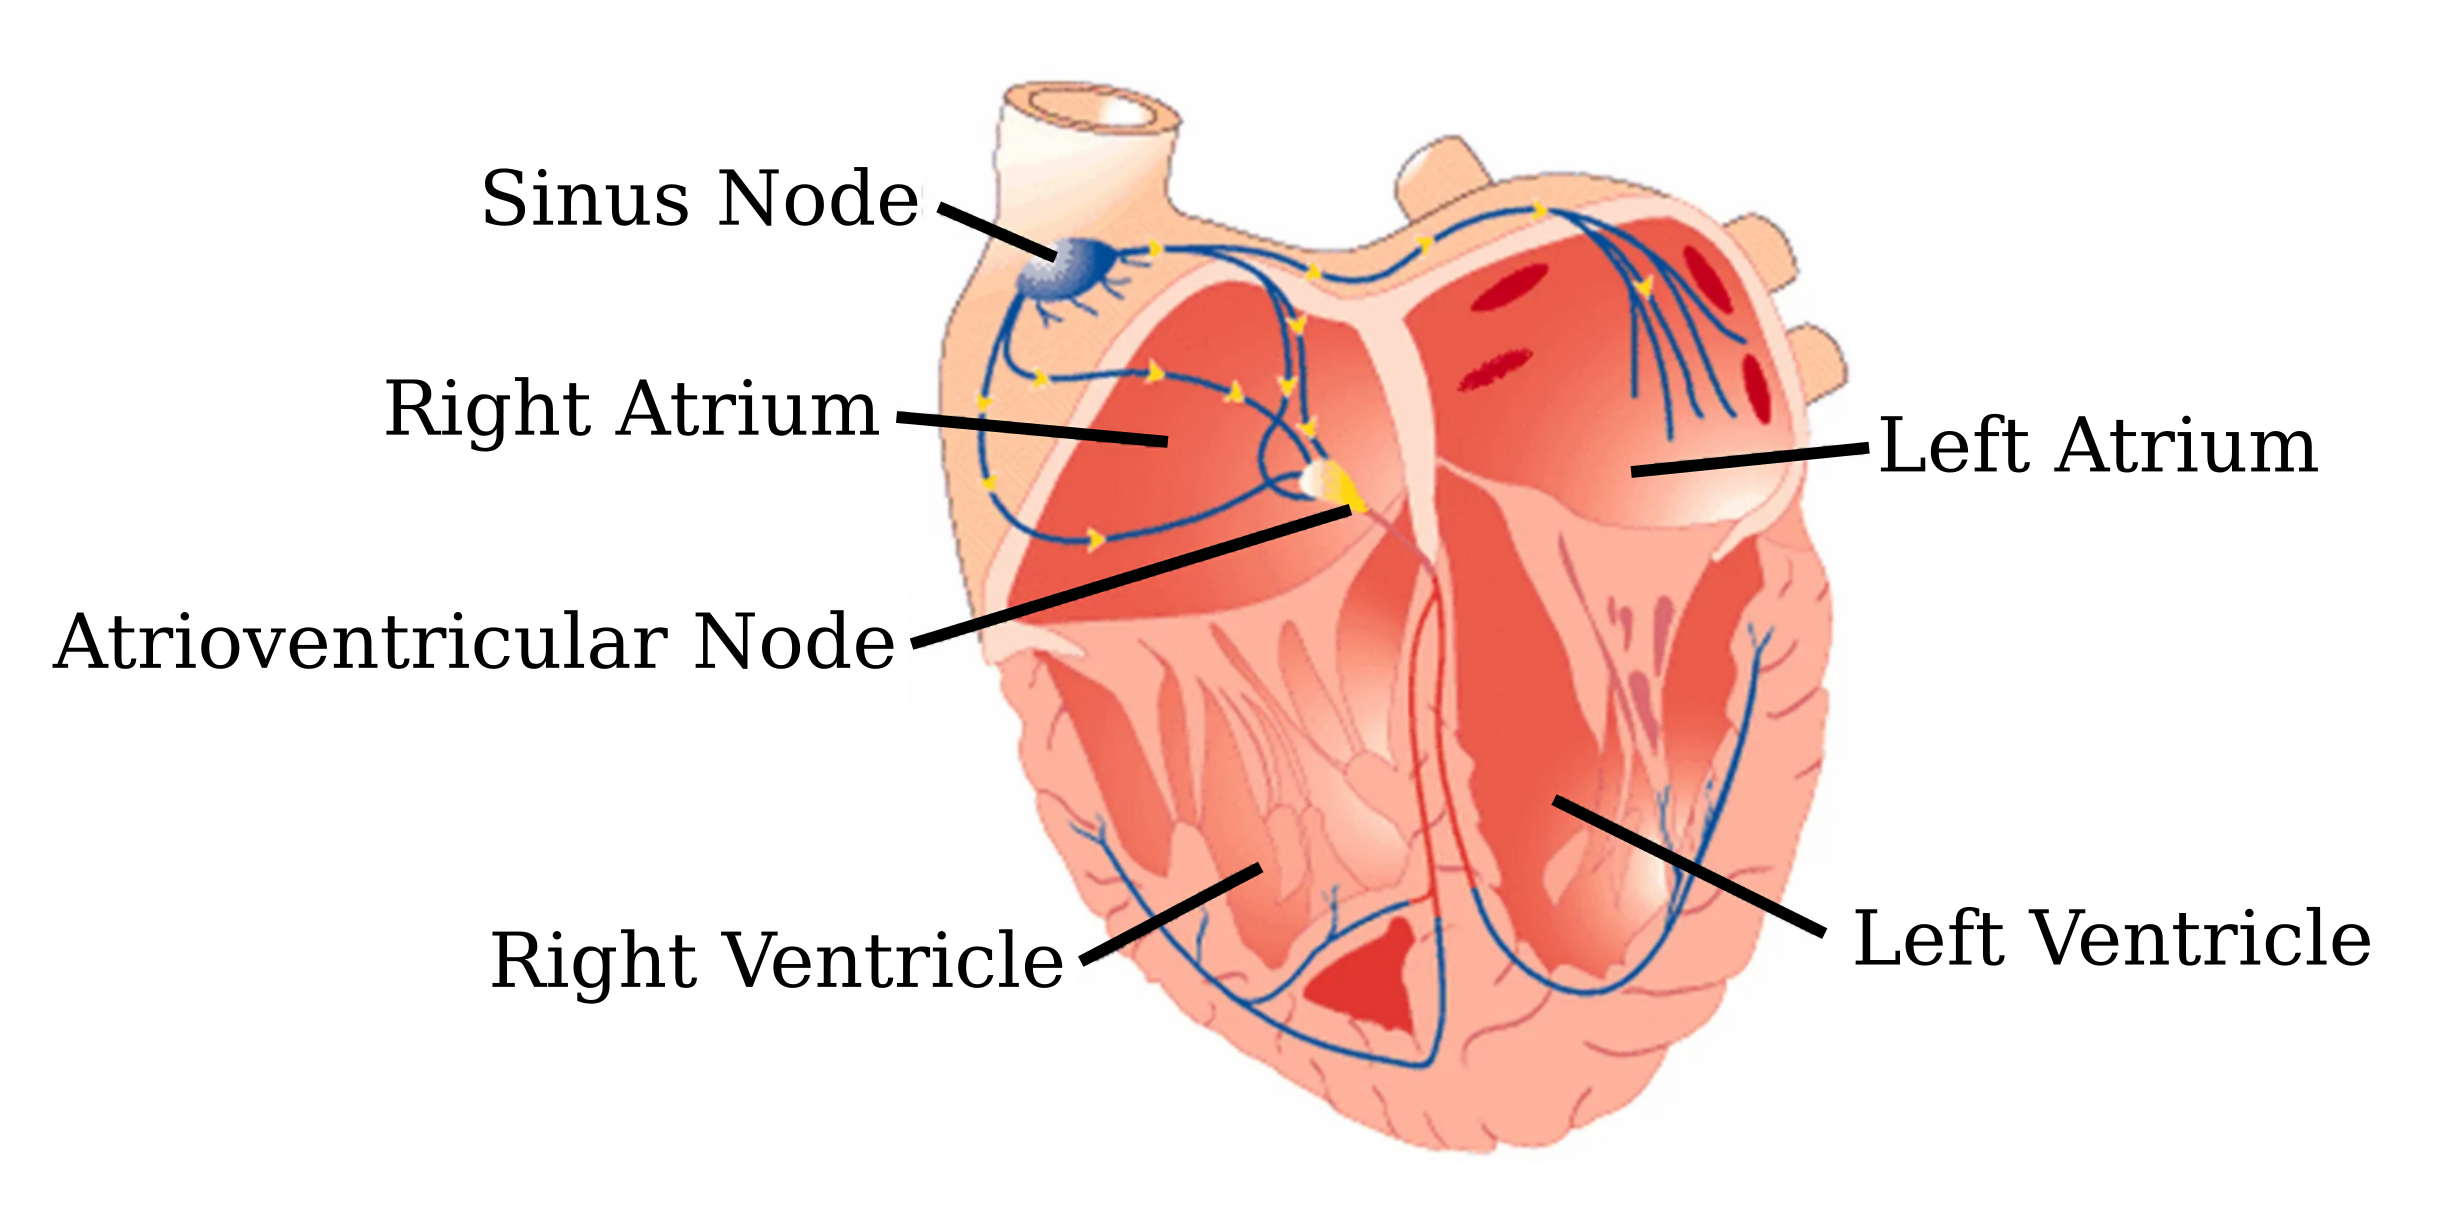
\includegraphics[width=1.0\textwidth]{figures/heart_physiology.png}
	\caption{Anatomy of the heart with the four chambers (two atriums and ventricles) including the sinus and atrioventricular node. Copyright 2019 by a-fib.com}
	\label{fig:heart_anatomy}
\end{figure}

\subsubsection{Electrophysiology of cardiac cells}
% Signalweiterleitung
% 
The action potential causes the heart muscle cells to contract and transmit the signal to other neighboring heart cells. This transmission of stimuli results in a coordinated extraction of the heart in the normal state, which results in a pumping action, the heartbeat.

% Signalverarbeitung 
% 1. Transmembranecurrent


%Cardiac cells (cardiomyocytes) are the smallest functional unit of the heart. An electro-chemical signal propagates through gap junctions between cardiomyocytes and let them contract individually but coordinated, that the heart shows a pump effect.
%In figure (\ref{fig:cardiac_excitation}) the temporal progression of three interdependent processes are sketchily shown. The blue curve shows the action potential, a temporary characteristic deviation of the membrane potential of a cell, from the rest potential. The potential is dependent on the ion-concentration within the cell. The red line shows the Calcium transient which is indirectly responsible that the cell contracts, by activating myofilaments (proteins). The Calcium-ion channel is only one kind of multiple channels to control the potential in terms of polarization, hyperpolarization or depolarization \cite{mycardium_lecture}.
%The dotted green line shows the intensity of contraction, which is a delayed reaction of the action potential course. Their temporal dependent behavior is called excitation-contraction coupling (ECC).  On the other hand it is signaling receptors\footnote{DHPR-receptor (Dihydropyridine receptor), it is a Calcium-dependent channel and functions as a voltage sensors, for further information see \cite{woodcock_cardiomyocytes_2005}.} to prevent the cell from further Calcium-ions (Ca$^{2+}$) to get into the cell. With exchanging Calcium-ions, the cardiomyocytes 'communicate' with each other, and allow the actions potential to be transferred that they act as an electrical neighbors-wise coupled system and are able to contract coordinated.
%The action potential has a refractory period where it does not show any response to a stimulus from another cell, which lasts around 250 milliseconds, to protect the heart. This period is relatively long in comparison a nerve cell, which has a refractory period of around 2 milliseconds. 


% Cells as smallest units, explaining a bit

% 


\begin{figure}[ht]
    \center
    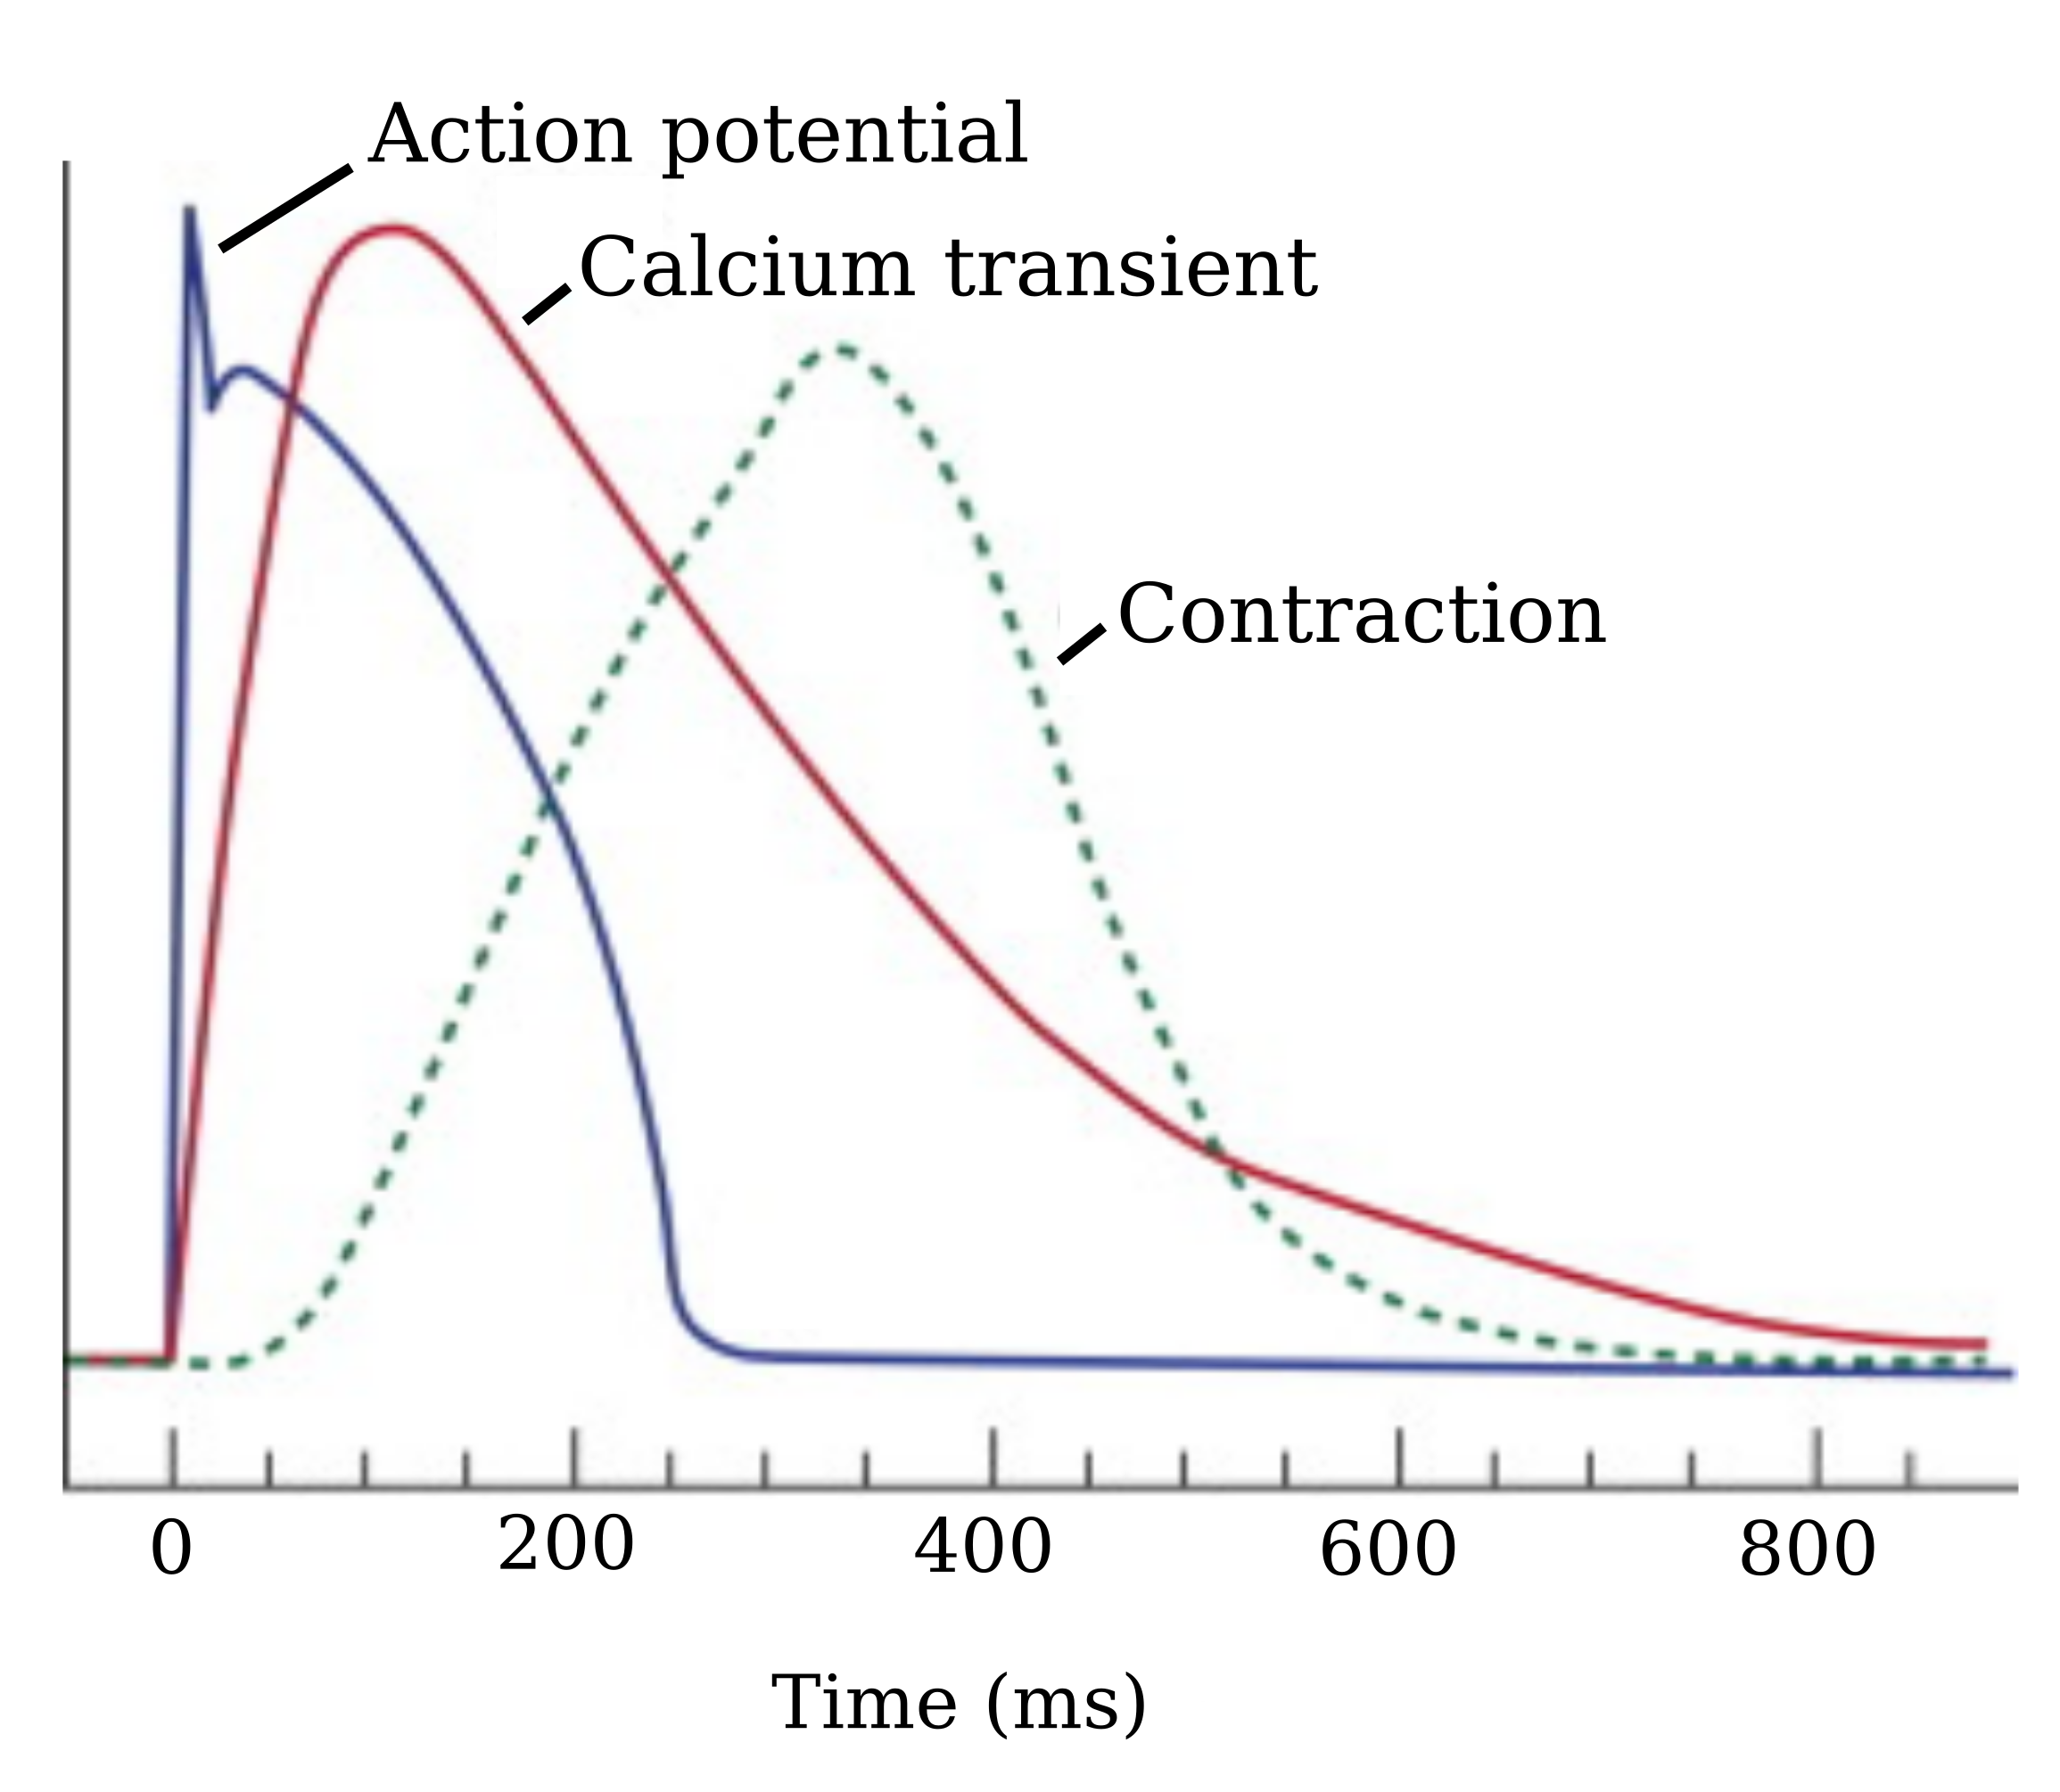
\includegraphics[width=0.7\textwidth]{figures/caradio_excitation.png}
	\caption{Physiology of the heart. Copyright 2020 by sciencedirect.com}
	\label{fig:cardiac_excitation}
\end{figure}

\section{Electrocardiography}
% In broad terms: what?
The electrocardiography is a representation of the heart's electrical activity, measured at a certain distance from the heart. The representation is in the form of potential differences, whereas the potentials are measured with the help of electrodes on the body surface. By subtracting the measurement of one electrode (or virtual electrode) with another as reference, one can gain information about the spatial potential gradient along the vector between both.
A pair of electrodes form a so called lead, by subtracting one signal from the other as a reference. A lead can be partially or fully made up of virtual electrodes, where the term virtual is used, as far as if a measurement is build from the average potential from multiple electrodes. A virtual electrode represents the potential at the spatial average of other electrodes of which it is built.
A widely known setting is the 12-lead-ECG, where 10 electrodes are used to form 12 leads. The positioning of these is visualized in figure (\ref{fig:12-lead-ecg}). The leads form vectors of which 6 lie on a vertical plane (frontal leads) and 6 on a horizontal plane (transverse leads).

\begin{itemize}
    \item Frontal leads have in common that one electrode is ideally placed (virtually) inside the heart. With the second electrode, which is marked on the image (\ref{fig:12-lead-ecg}) as V1, ...V6 (depending on the lead). The structure makes it possible to measure the potential difference between the inside of the heart and the surface of the body.
    \item Transverse leads
\end{itemize}
Here, a virtual electrode is built from \textbf{R}, \textbf{L} and \textbf{F}. It defines pairwise with V1 to V6 the first 6 leads.

\begin{figure}[ht]
    \center
    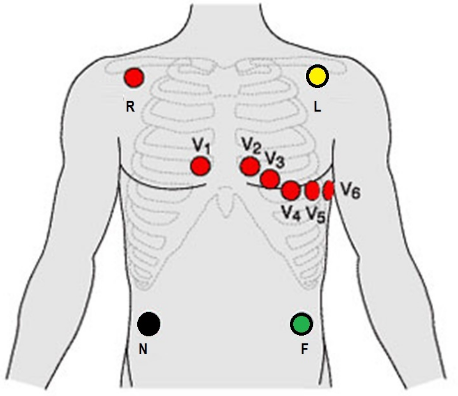
\includegraphics[width=0.7\textwidth]{figures/ecg_12_lead.png}
	\caption{\textcolor{red}{12-lead ECG, positioning. Copyright 2020 by firstaidforfree.com}}
	\label{fig:12-lead-ecg}
\end{figure}

The propagation of the electrical signals from the heart to the surface can be modeled as a diffusion process (also simulated in this work as such). This process is topic of the next chapter.
%The 12-lead ecg is designed to cover a variety of


%In conclusion, the ECG allows to measure a set of potential differences between two points at the body. By defining leads through two electrodes, a potential difference can be measured along a spatial vector. In the 12-lead ECG setting, the leads are placed such that 6 of these span vectors from the heart toward the torso. 

%The experiment as well considers though the choice of the reference electrode a 

\subsection{Forward propagation from the heart}
The terminology forward and inverse suggest that there is a direction in which the signals propagates. The suggestion here is that the potential differences lead to  
\section{The inverse problem}


\subsection{Related work and limitations}


\section{Simulation of ECG signals}\label{cap:simulation}
The following is a description of the simulation of a heart-model and its corresponding ECG signals.
The electrical activity of the heart is simulated with the FitzHughNaguro model on a pig's heart where the 3D structure is based on a computed tomography scan (CT-scan). Two grids of electrodes are placed at a certain distance from two opposing sides as visualized in figure (\ref{fig:pig_heart_in_bath}). 
The following data are considered in the numerical experiment: 
\begin{itemize}
    \item The activity of the heart model at each discrete point in the form of a system parameter (see chapter 1000).
    \item The potential differences of the respective electrodes of the grid, to a virtual electrode at the approximate center of the heart.
\end{itemize}
 

The simulation-framework is provided by Baltasar Rüchardt where the generation of the data can be divided into 4 parts, which I will describe below.\\

\textbf{1. Simulation of excitable media (electrical activity of the heart)}\\
Hey\\

\textbf{2. Reconstruction of the extracellular potential in the heart}\\
hey\\

\textbf{3. Diffusion process in the bath}\\
hey\\

\textbf{4. Calculation of the ECG}\\


%To generate ECG signals, the model for the activity in terms of extracellular potential of the heart is based on a pseudo-bidomain model. Especially when simulating an ECG the bidomain formulation is considered to be the most detailed biophysical approach \cite{bishop_bidomain_2011} but computational cost intense. To reduce the cost, the model includes the assumption, the intra- and extracellular domains to be anisotropic, but to the same degree. The bidomain model is then simplified to the mentioned pseudo-bidomain model, so that for the extracellular potential the equation 
\begin{align}
    C_m\frac{\partial V_m}{\partial t}+I_{\text{ion}}=\nabla(\sigma_m\nabla V_m)
\end{align}
applies, where $C_m$ is the membrane capacitance per unit area, and $I_\text{ion}$ is the ionic current density through the membrane. The parameter $\sigma_m$ can be regarded as bulk conductivity\footnote{For further derivation and explanation see \cite{bishop_bidomain_2011}.}.

The local ion flux is simulated with the FitzHugh-Nagumo model \cite{fitzhugh_1955}.

The 3D model of the pig-heart consists of around 32000 connective points to define a finite element mesh. The differential equations are solved with help from the open-source framework DOLFIN \cite{LoggWells2010a} in Python, the FitzHugh-Nagumo equations are solved by the implementation of the Runge-Kutta solver from scipy \cite{2020SciPy_NMeth}.

The main simulation framework is provided by Baltasar Rüchardt \cite{baltasar} and contains four steps:\\
\begin{itemize}
    \item augmented monodomain simulation,
    \item reconstruction of the extracellular potential in the heart,
    \item diffusion process in the bath,
    \item calculation of the ECG.
\end{itemize}

The potential propagates as a diffusion process through the bath, it can be regarded as a process which blurs the propagating potential. In the last step, because each electrode contains multiple points, the signal is integrated over each of these subsets. Figure (\ref{fig:pig_heart_in_bath}) shows the simulation setup with the heart inside the bath with the included ECG-electrodes, attached on the two panels from two sides.

\begin{figure}[ht]
    \center
    \hspace*{-2.45cm} 
    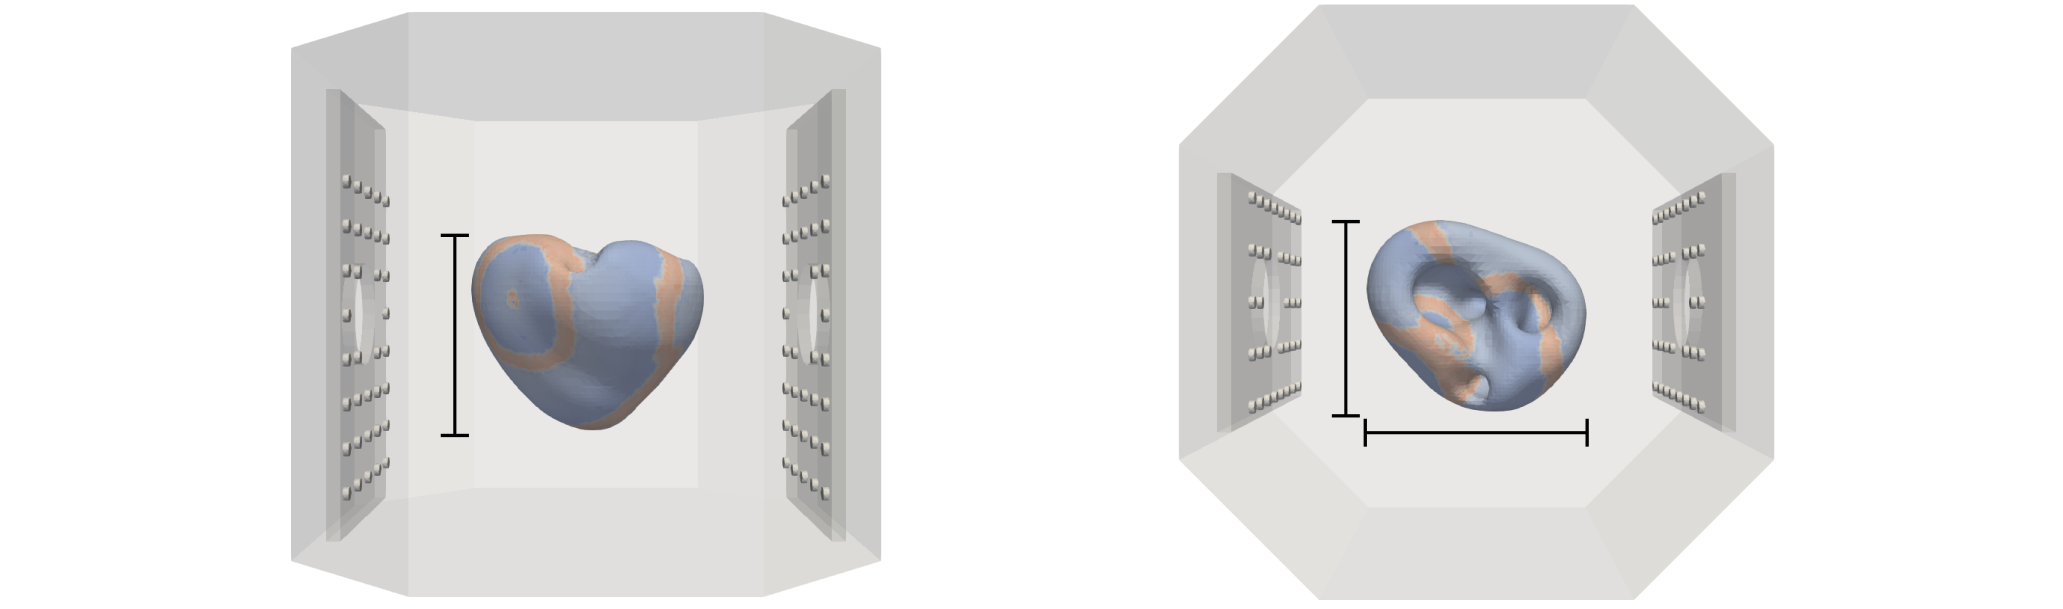
\includegraphics[width=1.4\textwidth]{figures/simulation_setup.png}
	\caption{Simulation of a pig heart, visualized with paraview \cite{paraview}, the panel on the left and right side on each image contain 64 electrodes for the simulated electrocardiography, as they are placed in the experiment in \ref{cap:concentricwave}.}
	\label{fig:pig_heart_in_bath}
\end{figure}

\section{Machine learning for iECG problem}

\begin{figure}[ht]
    \center
    \hspace*{-2.45cm} 
    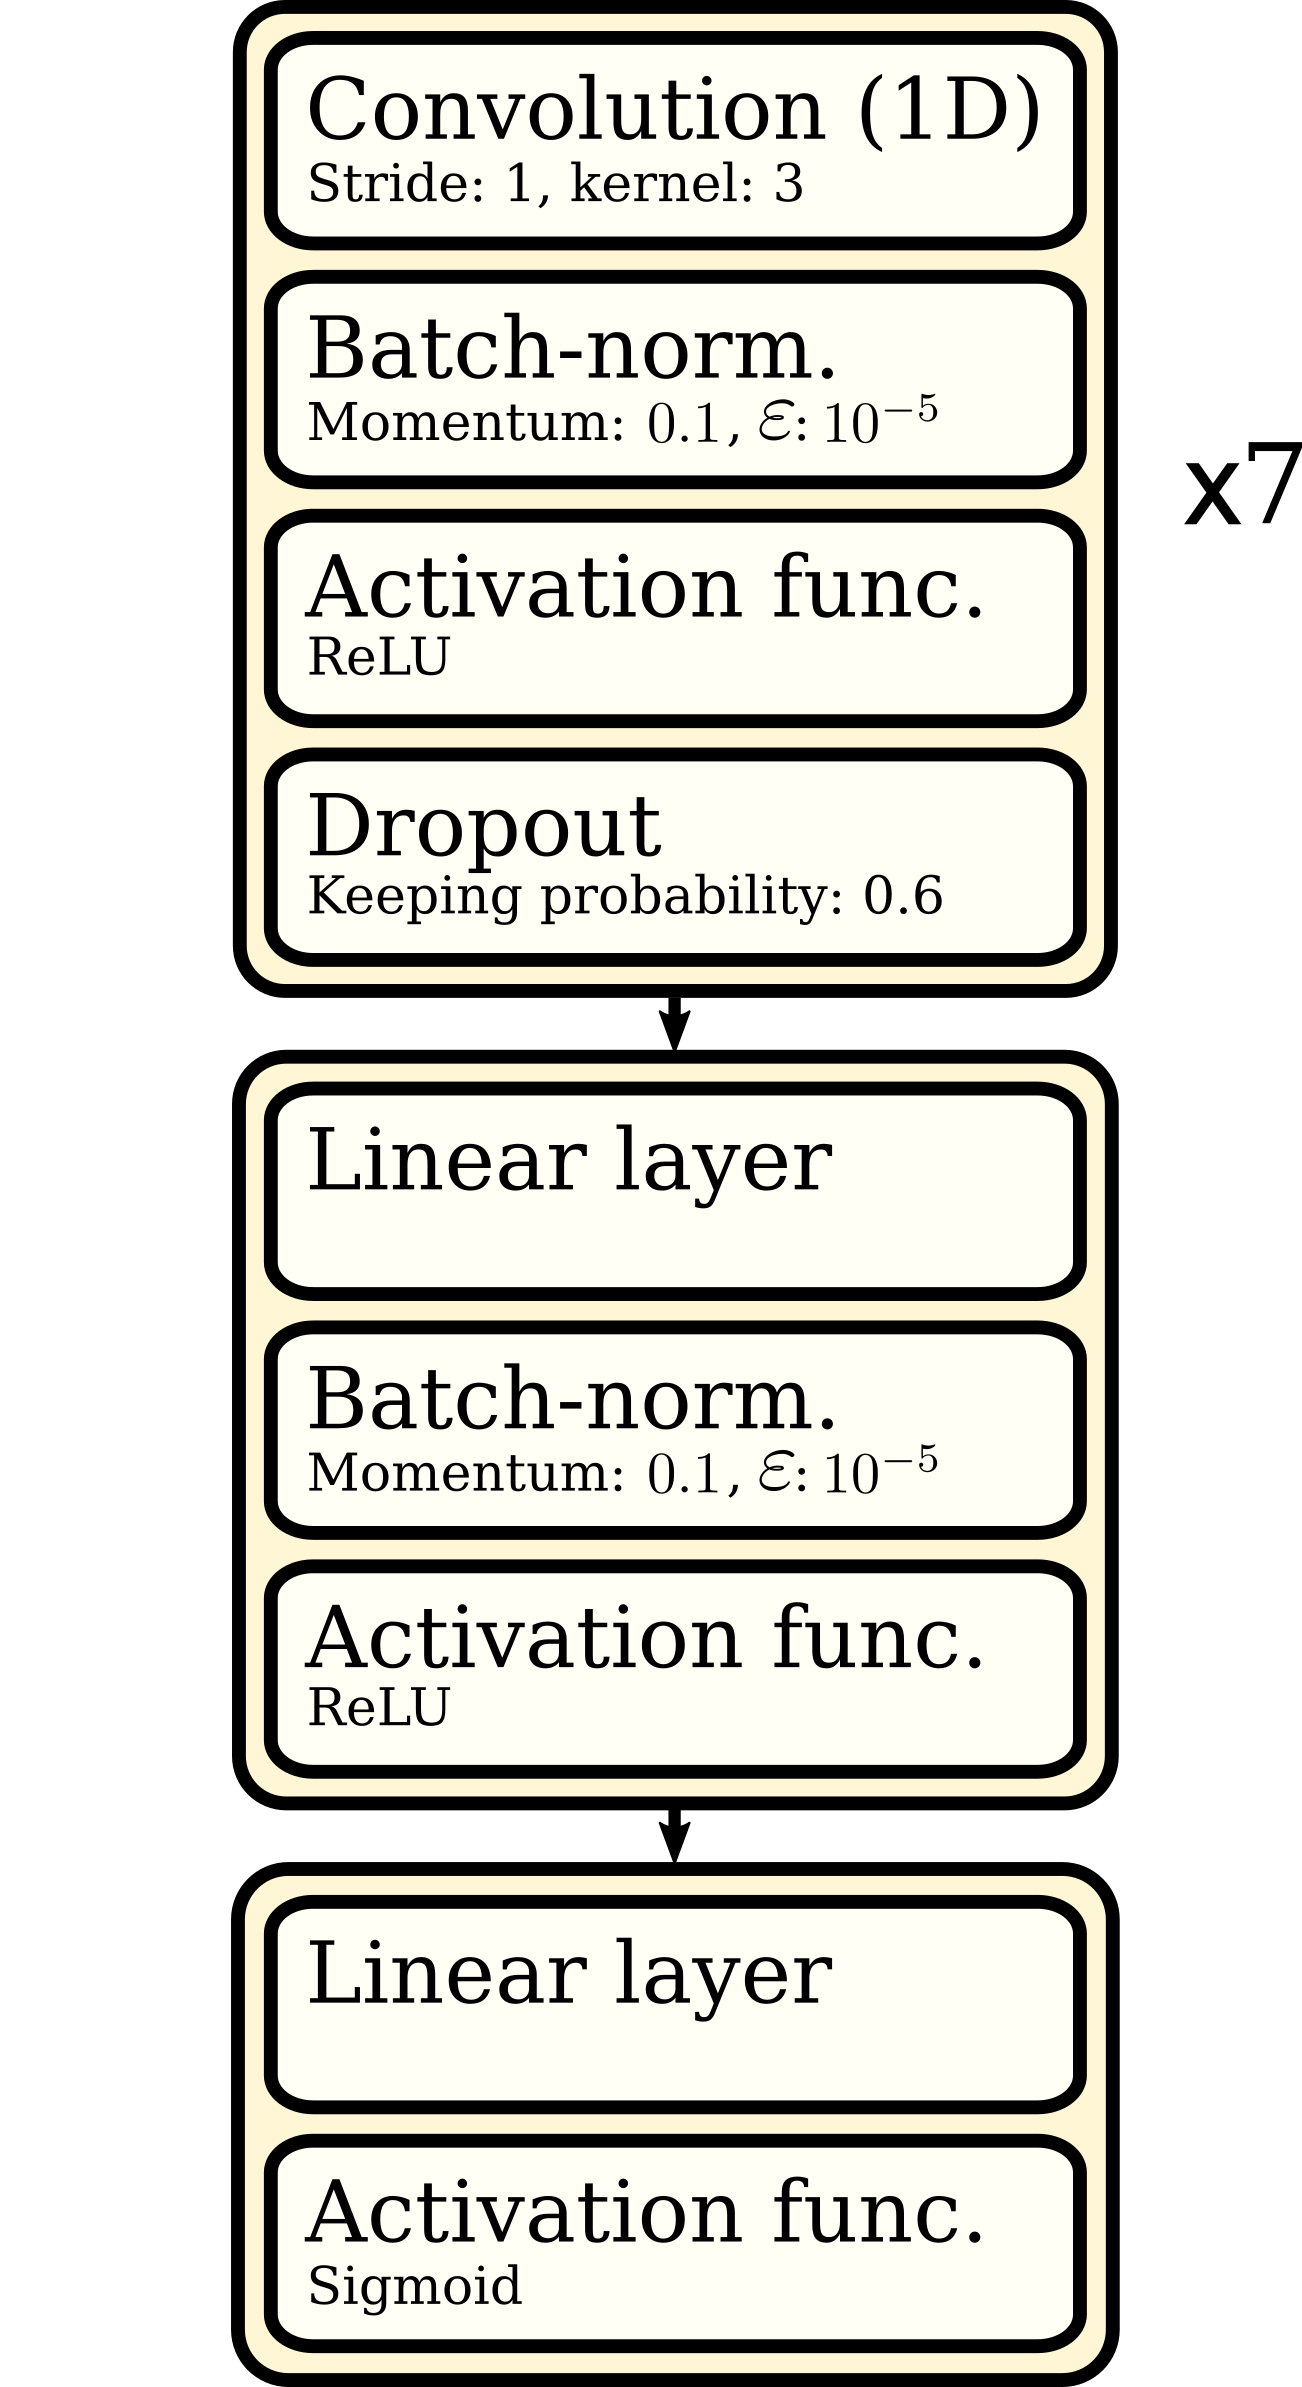
\includegraphics[width=5cm]{figures/ecg_cnn1d.png}
	\caption{}
	\label{fig:pig_heart_in_bath}
\end{figure}




\subsection{Data processing}\label{cap:processing}


\subsection{Neural network approach}

\section{Results and validation}
In the following I present the performance of the convolutional neural network (c.f. section \ref{convnet}) which is trained to predict the source of a concentric.
\subsection{Concentric Wave Localization} 
With the regularization methods during the training process (c.f. section \ref{cap:concentricwave}), the training lasted for 2310 epochs. This took around 58 minutes on a Nvidia K100 GPU. While the heart has an expansion of between around 60 and 80 length units, the model is able to predict the source of the concentric wave from the validation set on average with a displacement of 3.11 length units. Imagine a pig's heart which was simulated, and estimating the size of the heart of between 10cm and 20cm in each direction (x, y, z), the average displacement would be approximately between 0.75cm and 1cm. The comparability faces limitations due to the fact that the simulation produces a system without noise (geometrical noise in time and space, uncertainties on the measurements or positioning of the electrodes etc.) Nevertheless, it shows a first attempt that the CNN is able to localize the source of concentric waves (under the prerequisite of perfect conditions) from unknown data, whose displacement is not orders of magnitude worse when comparing with the results from the training-dataset.\\

\begin{table}[h]
    \centering
    \begin{tabular}{|c|c|}
    \hline
    training set & test set\\
    \hline
    1.74 & 3.11 \\
    \hline
    \end{tabular}
    \caption{Average displacement of the prediction from the CNN on the training- and test-dataset.}
    \label{tab:convarchitec}
\end{table}

\begin{figure}[ht]
    \center
    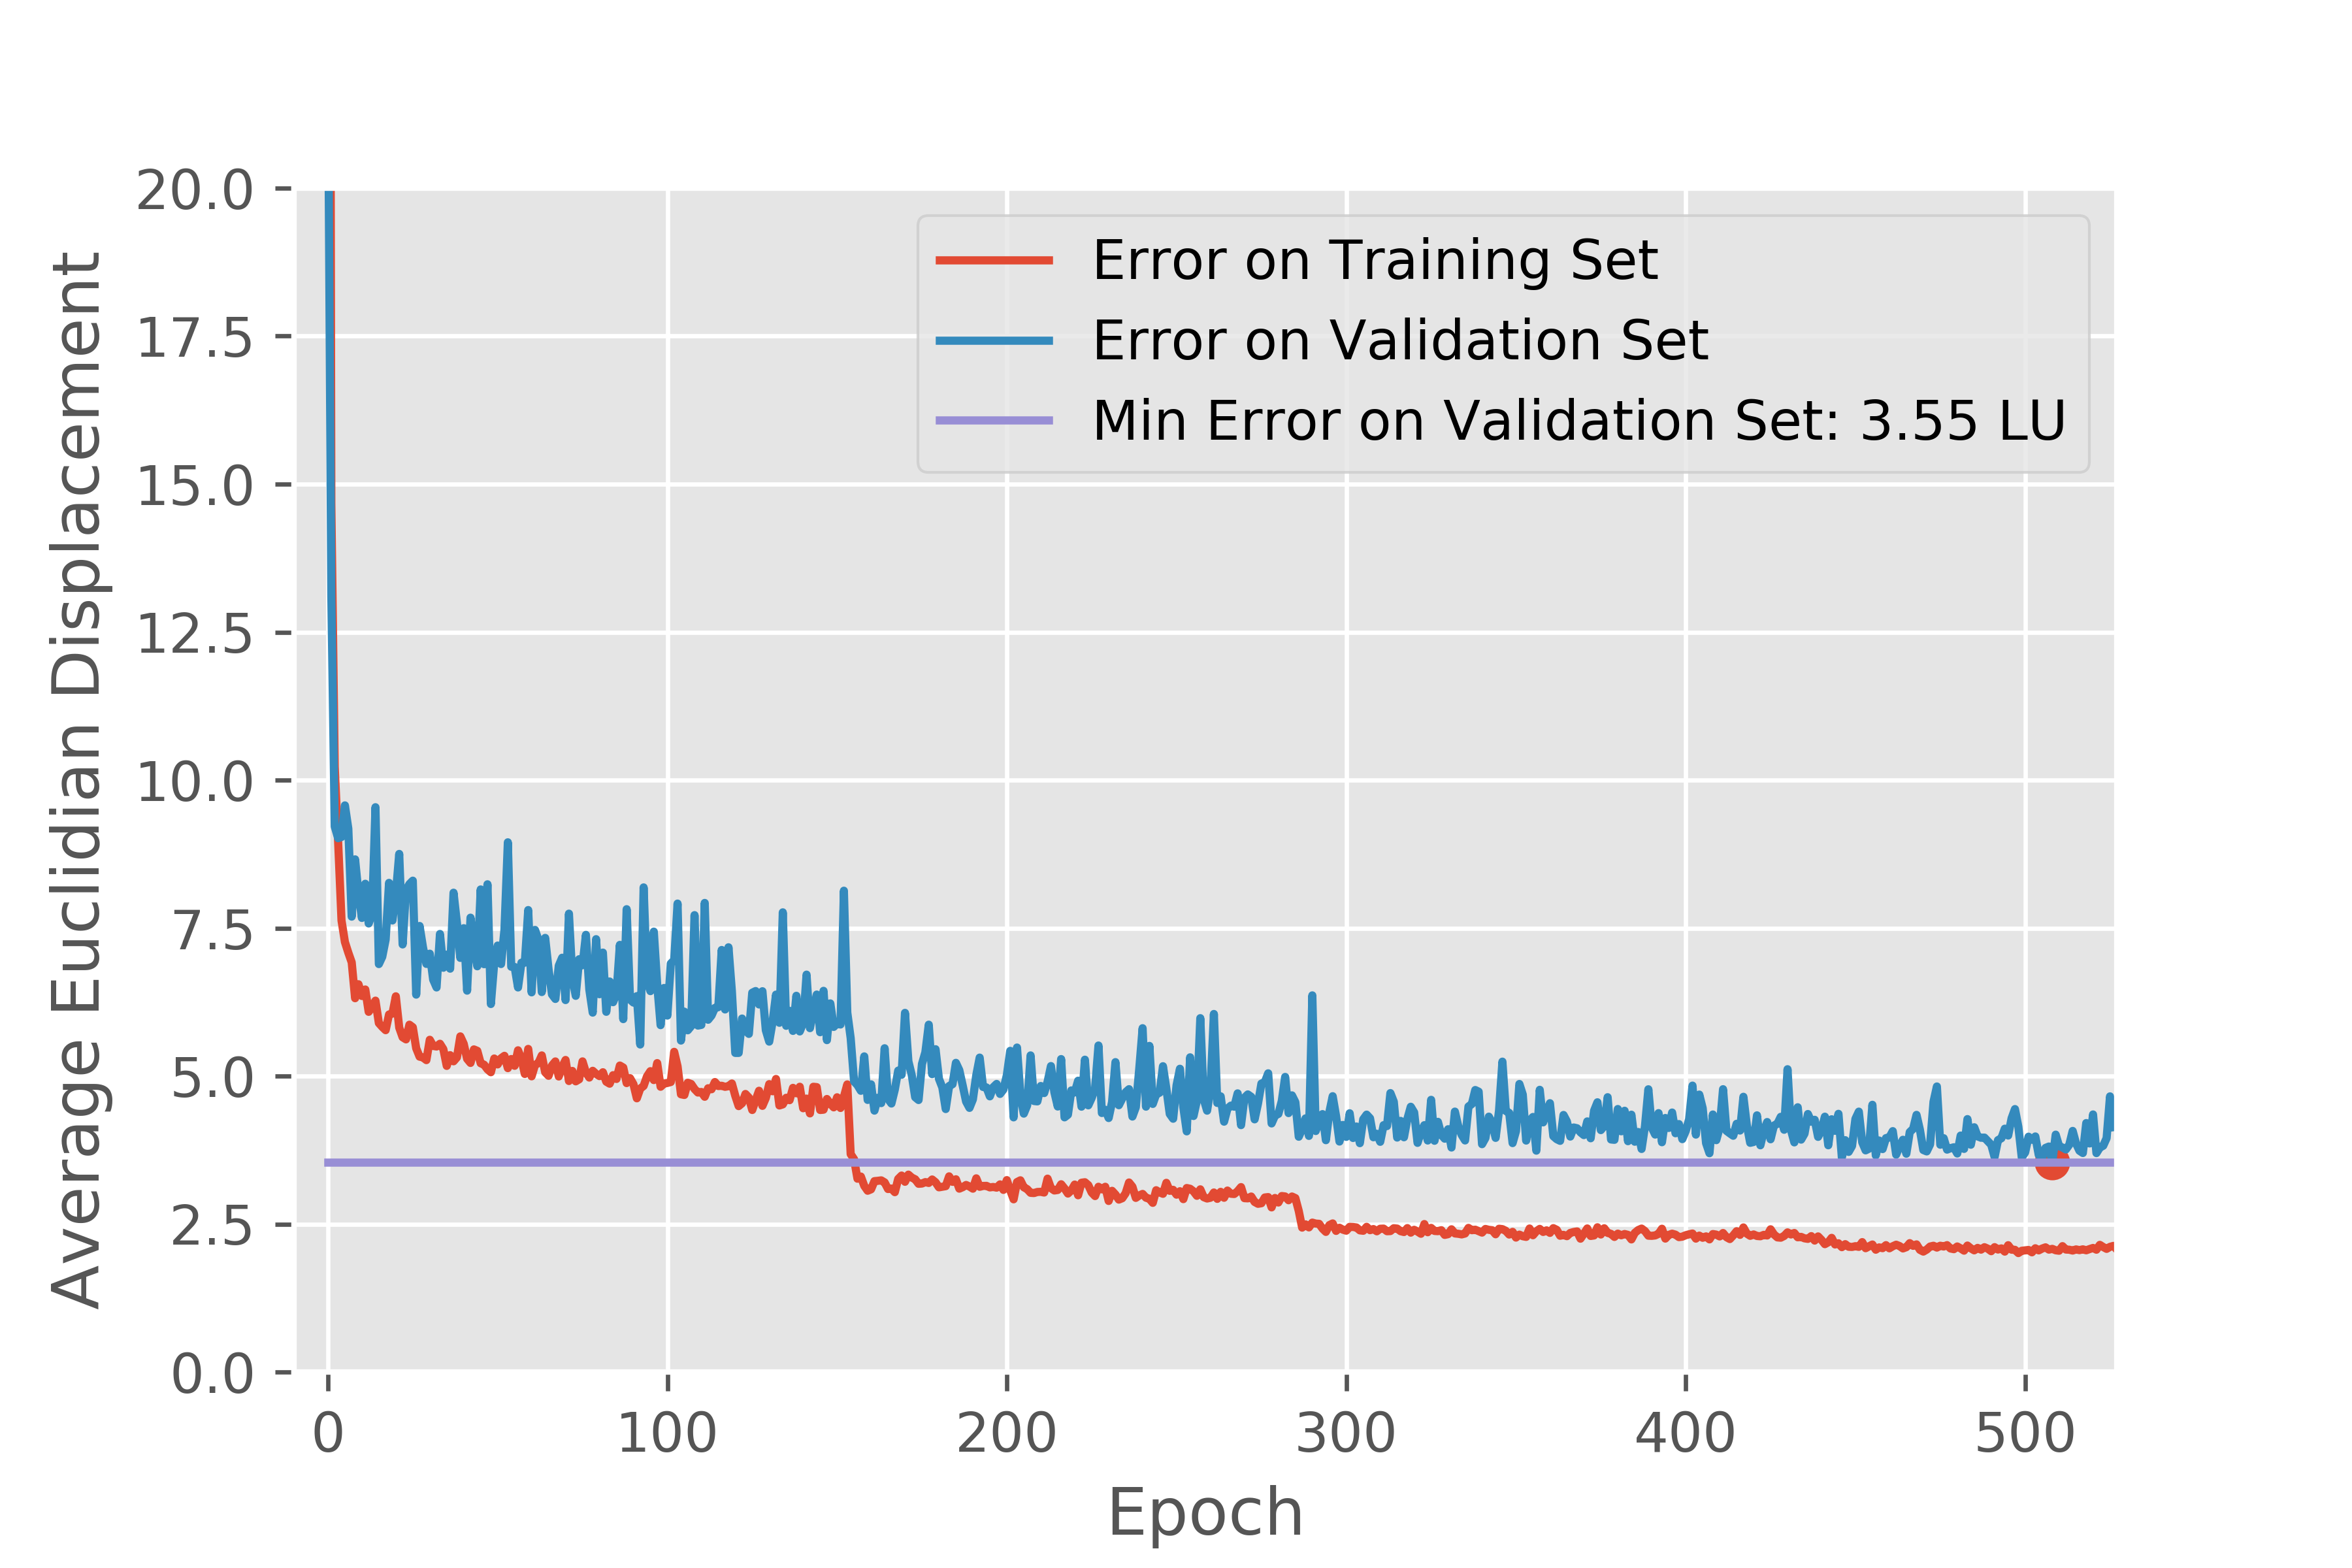
\includegraphics[width=0.99\textwidth]{figures/reg_plot1.png}
	\caption{Development of the average euclidean displacement by epoch on the training- and validation set.}
	\fontsize{3}{2}
	\label{fig:autoencoder_architecture}
\end{figure}

\subsubsection{Limitations of the Model}
This experiment is an attempt to show the principle ability to use convolutional neural network to solve a task with a time-series as input. This special posed task of the inverse problem of ECG gave comparably good results. This shows that the neural network is able to process through a temporally random selected section of fixed length, which makes it clear that it recognizes a pattern in the signals regardless of the phase of the concentric wave. The simulated heart contains of around 10000 elements on the surface, which can represent an approximate source of the concentric wave. While having 1024 simulation, having unique starting conditions, around 10\% of the available sources are already covered.  The properties of a simulation differ only in the location of the pacing events that cause the concentric wave. It is possible that some training and test simulations differ very little from each other, if the locations of the pacing events are very close to each other. In this case it may not be possible to speak of a truly unknown data set. The average minimal distance from a test-simulation to the next training-simulation is around 2.47 LU. It shows that the neural network is trained with pacing positions, which are not far distant from the test-simulations. Furthermore, the neural networks average displacement of the predictions on the test-dataset is bigger than the average distance to the next training simulation. Nevertheless, the same CNN is able to handle a dataset with additional Gaussian noise. The training on the same dataset with this noise with $\sigma=0.05$ got displacements as shown in table \ref{tab:noise}:

\begin{table}[h]
    \centering
    \begin{tabular}{|c|c|}
    \hline
    training set & test set\\
    \hline
    1.69 & 3.15 \\
    \hline
    \end{tabular}
    \caption{Average displacement of the prediction from the CNN on the training- and test-dataset, additional Gaussian noise with $\sigma=0.05$ is added to the normalized data (this means that a 5\% error is included).}
    \label{tab:noise}
\end{table}

The average displacement on the test-dataset did not increase much (a difference of 0.04LU).
